\documentclass[10 pt]{beamer}
\usetheme{Madrid}
\usepackage[utf8]{inputenc}

\usepackage{xspace}
\usepackage{graphicx,graphics} 
\usepackage{color}
\usepackage{amsmath}
\usepackage{mathrsfs}
\usepackage{amsfonts}
\usepackage{amssymb}
\usepackage{amsthm}
\usepackage{algorithm}
\usepackage{algorithmic}
\usepackage{longtable}
\usepackage{complexity}
\usepackage{tkz-graph}
\usepackage{float}
\usepackage{setspace}
\usepackage{multicol}
\usepackage{subcaption}
\usepackage[absolute,overlay]{textpos}
\graphicspath{{img/}}
\tikzset{
  LabelStyle/.style = { rectangle, rounded corners, draw,
                       font = \bfseries },
  EdgeStyle/.append style = {-} }
\title{Contention management for Deterministic Networking}

\author{DAVID,  Universit\'e de Versailles Saint Quentin}


\institute[Nokia Bell Labs, DAVID-UVSQ] 
{
 
\includegraphics [width=20mm]{logo_n-green.png}  \\
}

\subject{Theoretical Computer Science}

\begin{document}

\begin{frame}

  \titlepage

  \begin{textblock*}{2cm}(5mm,8cm) % {block width} (coords)

\includegraphics [width=2cm]{anr.png}
\end{textblock*}
  \begin{textblock*}{1cm}(27mm,7.85cm) % {block width} (coords)

\includegraphics [width=10mm]{imageetreseaux.png}
\end{textblock*}
  \begin{textblock*}{3cm}(40mm,7.85cm) % {block width} (coords)

\includegraphics [width=30mm]{logon.png}
\end{textblock*}
  \begin{textblock*}{6mm}(73mm,8cm) % {block width} (coords)

\includegraphics [width=6mm]{tparistech.png}
\end{textblock*}
  \begin{textblock*}{6mm}(80mm,8cm) % {block width} (coords)

\includegraphics [width=6mm]{tsudparis.png}
\end{textblock*}
  \begin{textblock*}{6mm}(87mm,8cm) % {block width} (coords)

\includegraphics [width=6mm]{tbretagne.png}
\end{textblock*}
  \begin{textblock*}{10mm}(95mm,7.8cm) % {block width} (coords)

\includegraphics [width=10mm]{logod.png}
\end{textblock*}
 \begin{textblock*}{13mm}(107mm,8cm) % {block width} (coords)

\includegraphics [width=13mm]{iii-vlab.png}
\end{textblock*}
  %
\includegraphics [width=15mm]{logod.png} \hspace{1cm} 
\includegraphics [width=20mm]{logon.png} \hspace{1cm} 
\includegraphics [width=20mm]{logo_n-green.png} \\
\end{frame}


\begin{frame}{Problematic }
\begin{itemize}
\item Latency critical application (C-RAN, ....).
\item Stochastic networks could not ensure a low latency.
\item $\NP$-hard 
\end{itemize}



 \begin{block}{Periodic Process}
 
\begin{center}
   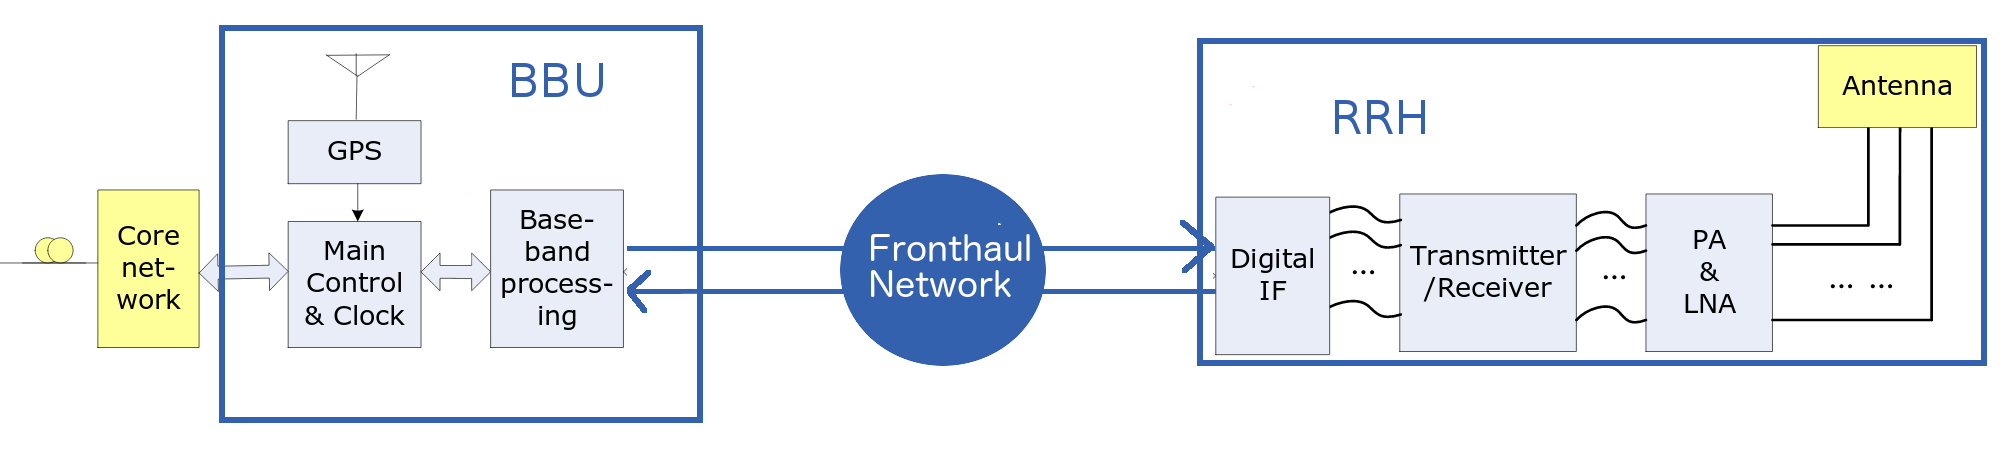
\includegraphics[scale=0.15]{BBURRH2.png}

    
\begin{itemize}
\item Contention in the fronthaul network
\item Need to guarantee the latency
\end{itemize}
 \end{center}
 
 \end{block}

 
 \end{frame}

 \begin{frame}
 \begin{center}
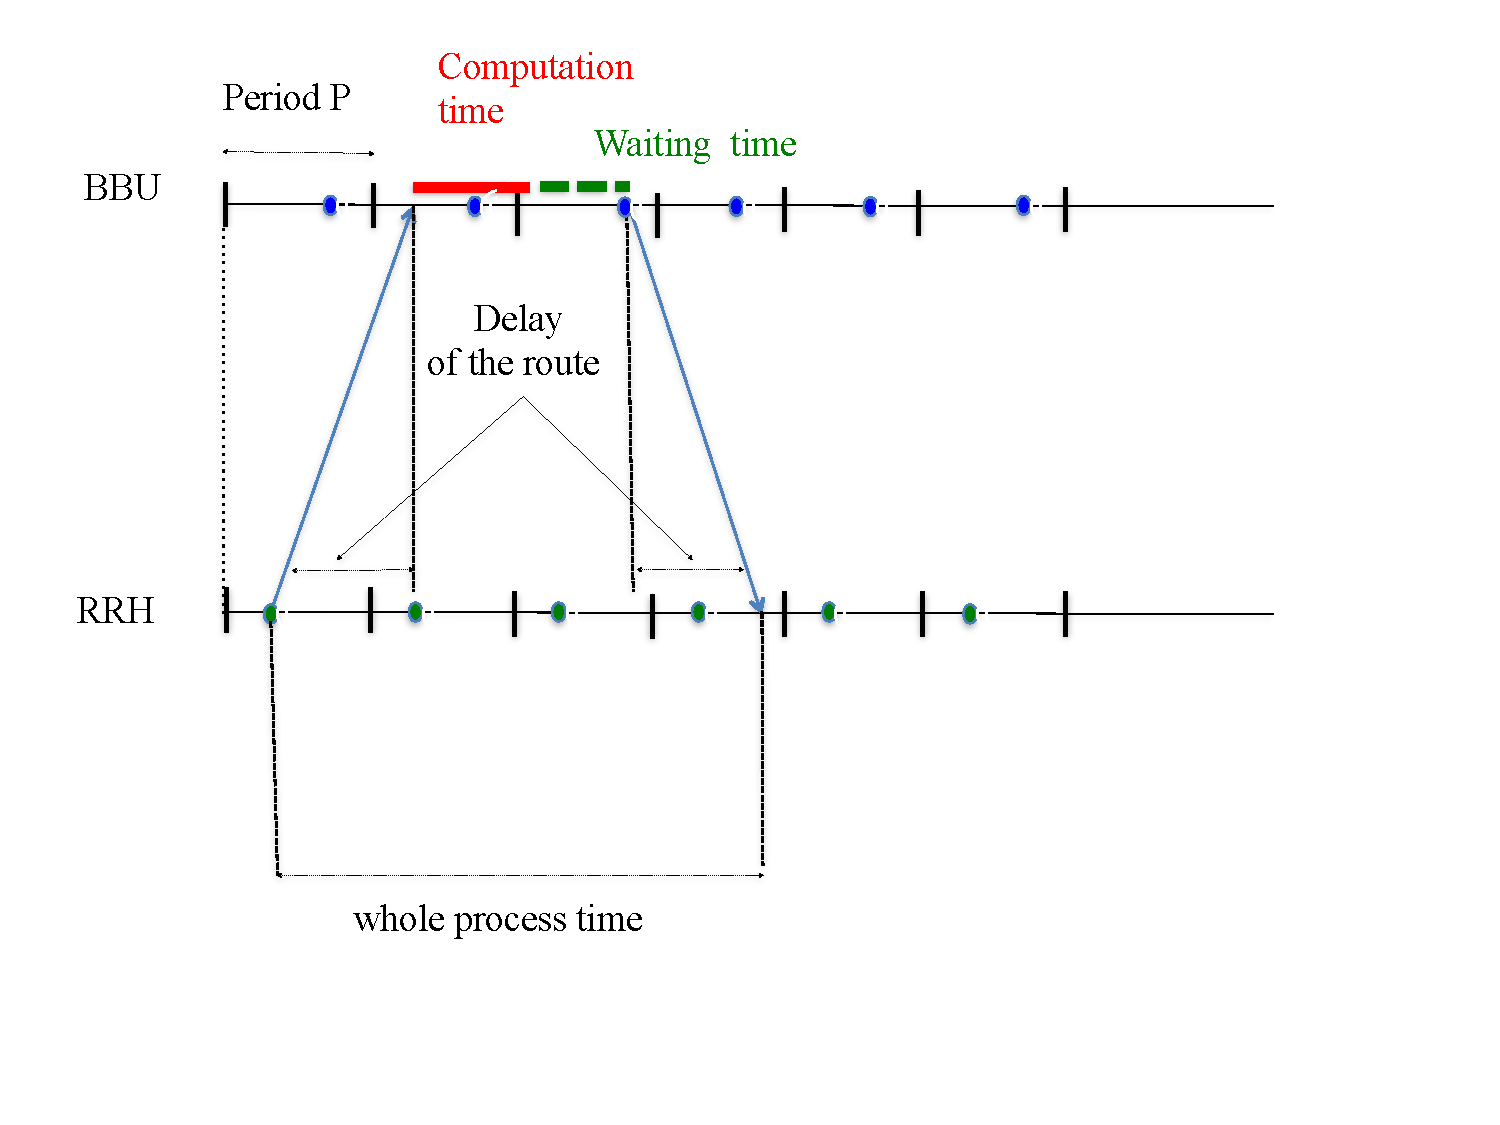
\includegraphics[scale=0.5]{periodic_process.pdf}

\end{center}
 \end{frame}

  
  \begin{frame}{Theoretical results}
  

\begin{block}{Problem}
Find some time at which send the messages from the BBU/RRH, such that there is no collisions in the network.
\end{block}

\begin{block}{\NP-hard}
On general topology, even with restricted parameters.
\end{block}

\begin{block}{Star network}
  \centering
\scalebox{0.3}{
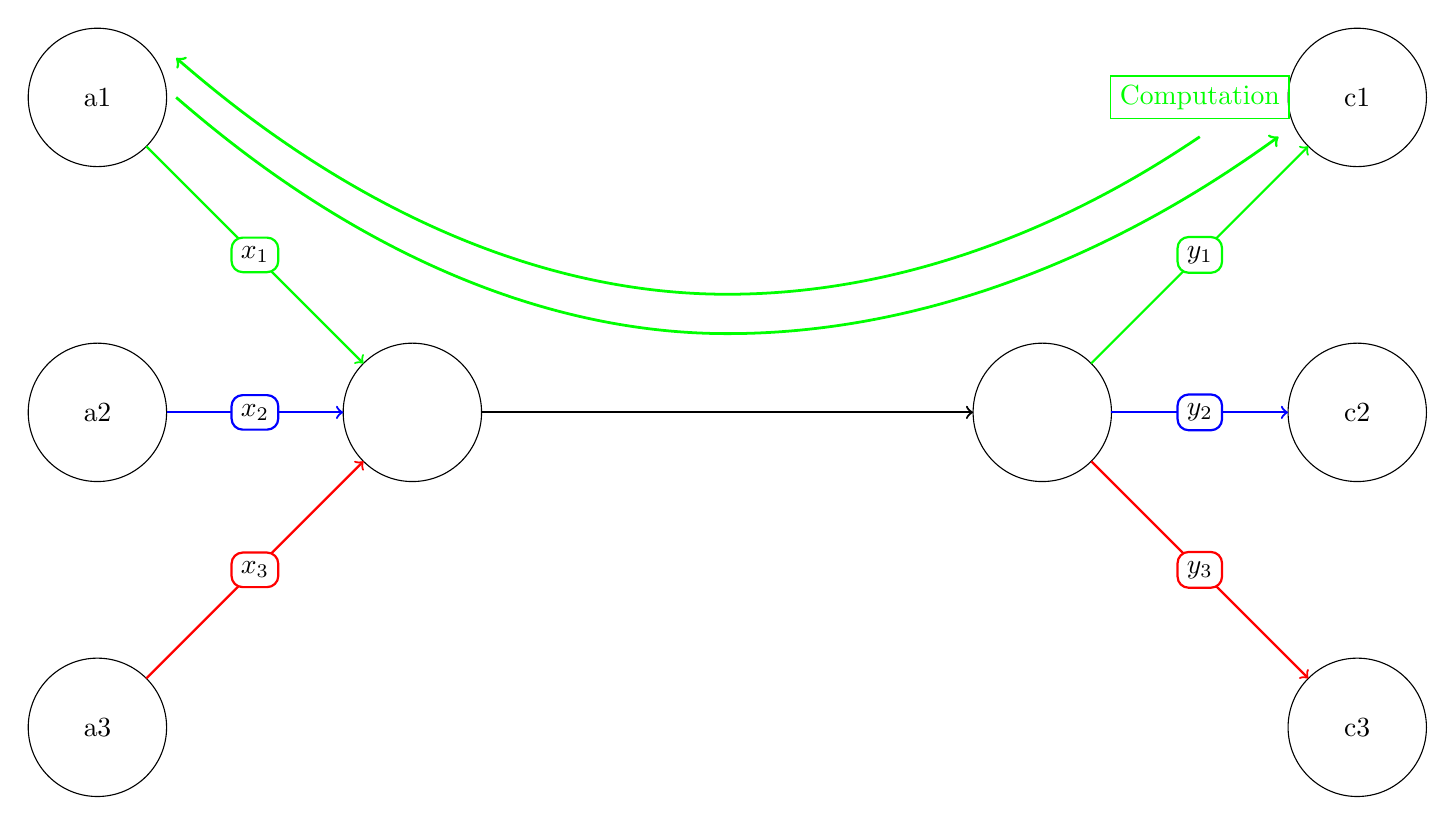
\begin{tikzpicture}
    \SetGraphUnit{5}
  \tikzstyle{VertexStyle}=[shape = circle, draw, minimum size = 50pt]
  \Vertex[x=0,y=0]{a3}
  \Vertex[x=0,y=4]{a2}
  \Vertex[x=0,y=8]{a1}
  
  \Vertex[x=16,y=0]{c3}
  \Vertex[x=16,y=4]{c2}
  \Vertex[x=16,y=8]{c1}
  
  \SetVertexNoLabel
  \Vertex[x=4,y=4]{SL}
  \Vertex[x=12,y=4]{SS}  
  \tikzset{
  EdgeStyle/.append style = {<-,green} }
  \Edge[label = $y_1$](c1)(SS)
  \Edge[label = $x_1$](SL)(a1)
  
  \tikzset{
  EdgeStyle/.append style = {blue} }
  \Edge[label = $y_2$](c2)(SS)
  \Edge[label = $x_2$](SL)(a2)
  
  \tikzset{
  EdgeStyle/.append style = {red} }
  \Edge[label = $y_3$](c3)(SS)
  \Edge[label = $x_3$](SL)(a3)
  
  \tikzset{
  EdgeStyle/.append style = {black} }
  \Edge(SS)(SL)
  
  \draw[->,line width=1pt,green] (1,8) parabola bend (8,5) (15,7.5);
  \node[draw,green] at (14,8) {Computation};
  \draw[<-,line width=1pt,green] (1,8.5) parabola bend (8,5.5) (14,7.5);


\end{tikzpicture}
}
\end{block}


\end{frame}




\begin{frame}{Optical ring}




\begin{block}{Model}
\begin{center}
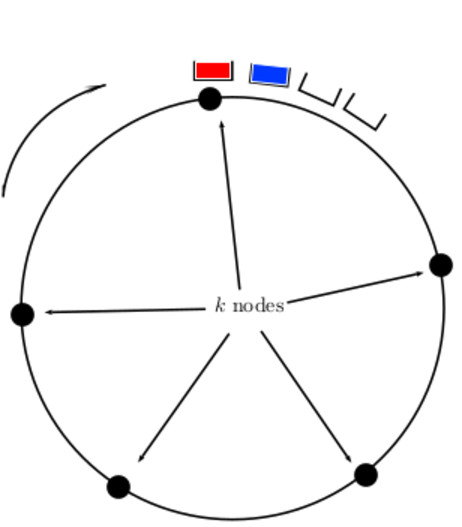
\includegraphics[scale=0.3]{anneau1.pdf}
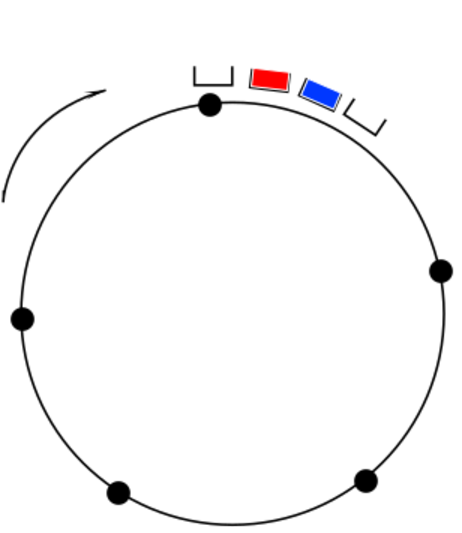
\includegraphics[scale=0.3]{anneau2.pdf}

Waiting only at the insertion
\end{center}
\end{block}

\begin{center}
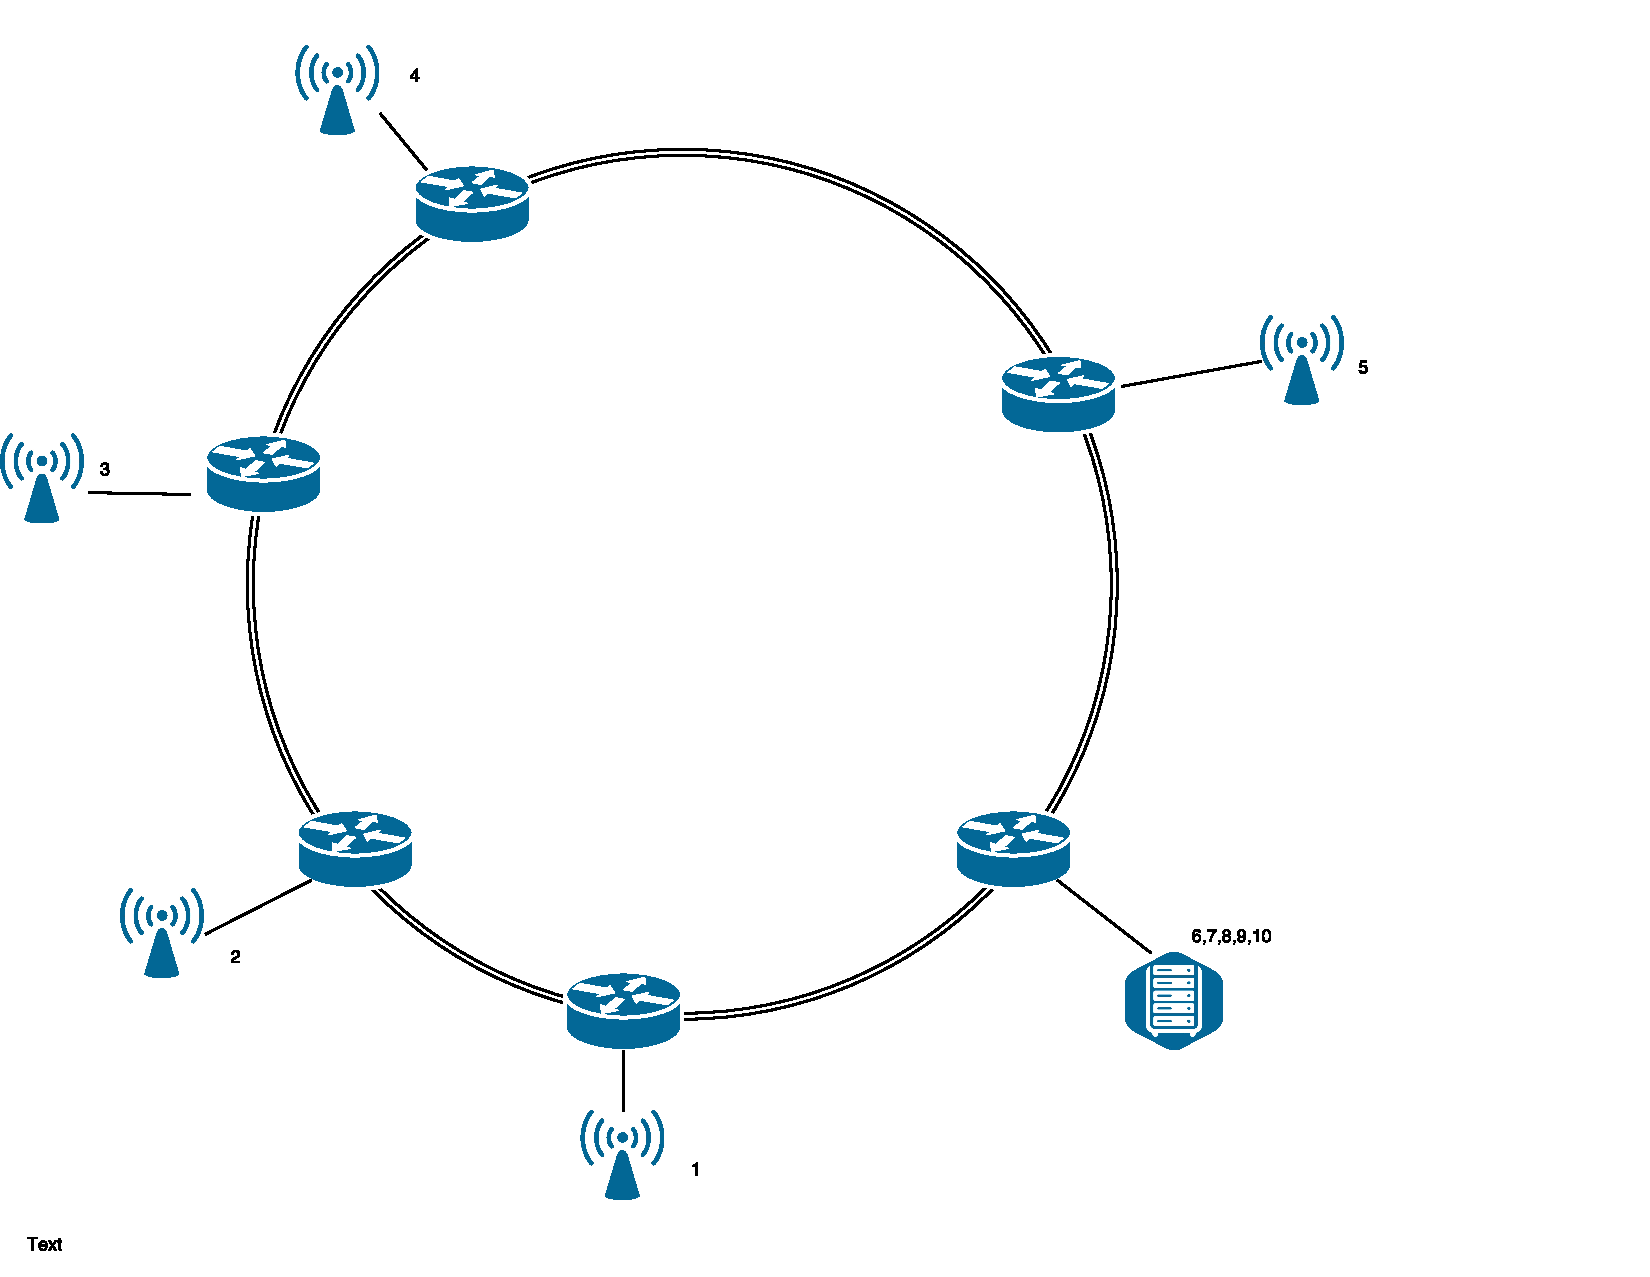
\includegraphics[scale=0.13]{anneau-simple.pdf}
\end{center}


\end{frame}


\begin{frame}{Insertion}


\begin{center}
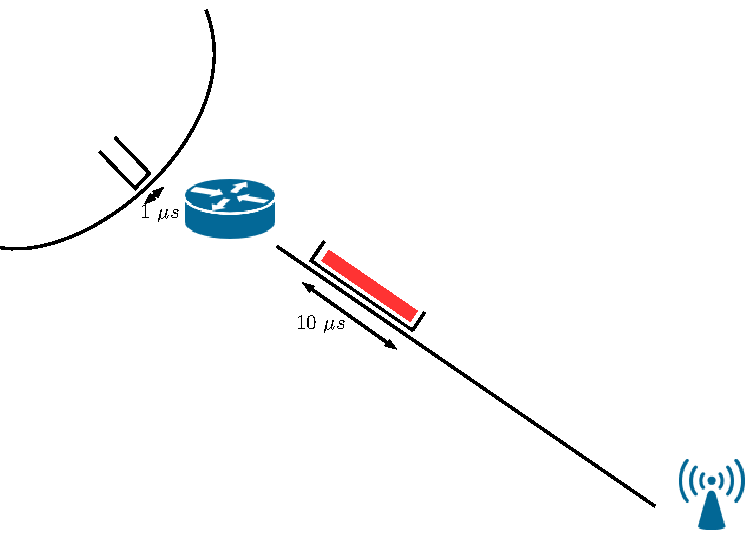
\includegraphics[scale=0.4]{slot1.pdf}
\hspace{1cm}
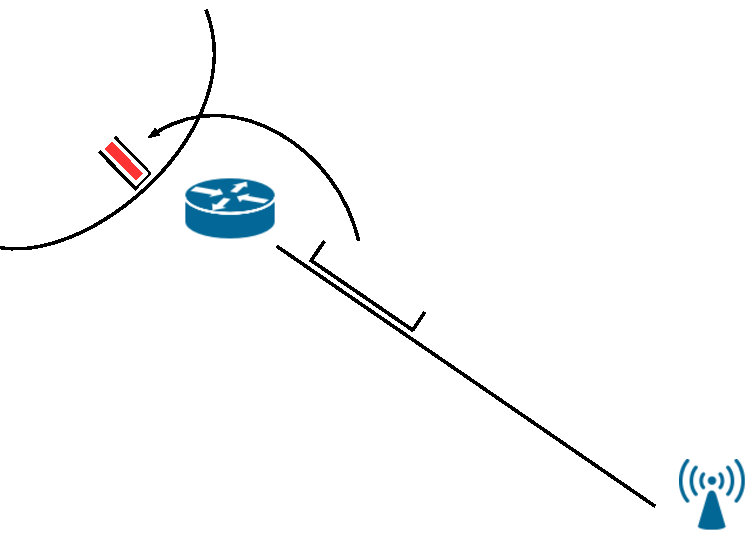
\includegraphics[scale=0.4]{slot2.pdf}

\end{center}

\end{frame}


\begin{frame}{Insertion}


\begin{center}
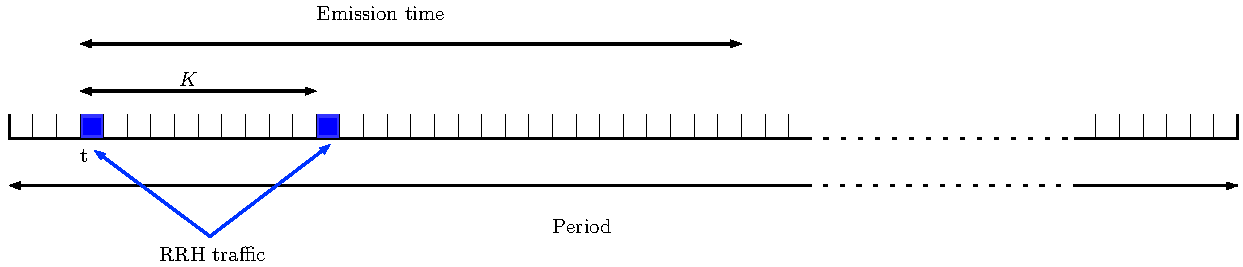
\includegraphics[scale=0.5]{emission_antenna.pdf}

\end{center}

\end{frame}




\begin{frame}{Parameters}
 \centering Broadcast and select Policy 
 
 
 \begin{block}{Parameters}
\centering
  \begin{tabular}{|c|c|}
  \hline
  Bit rate of an electronic interface $R$ & $10$ Gbps \tabularnewline
  \hline
  Optical ring bit rate $F\times R$ & $100$ Gbps \tabularnewline
  \hline
    Acceleration factor $F$ & $10$  \tabularnewline
  \hline
  Container size  $C$ & $100$ kb  \tabularnewline
  \hline
  Unit of time $C/(F\times R)$ & $1~\mu$s \tabularnewline
  \hline
  Length of the ring $RS$ & $100$ \tabularnewline
  \hline
  Emission time $ET$ & $500$ \tabularnewline
  \hline
   Period $P$ & $1,000$ \tabularnewline
  \hline
  Number of RRH & $5$  \tabularnewline
  \hline
  Number of nodes $n$ & $5$  \tabularnewline
  \hline
   Load induced by C-RAN traffic & $50\%$  \tabularnewline
  \hline
    Load induced by BE traffic & $40\%$  \tabularnewline
  \hline
  \end{tabular}

 \end{block}

\end{frame}

\begin{frame}{Optical ring problematic}
\begin{itemize}
\item We got two kinds of traffic : CRAN - high priority, Best effort
\vspace{1cm}
\item We want to observe the behavior of the ring and analyze the latency of CRAN
\vspace{1cm}
\item We will try to find some methods to decrease the CRAN latency without increasing the Best effort latency too much
\end{itemize}
\end{frame}

\begin{frame}{Opportunistic insertion policy }

\centering
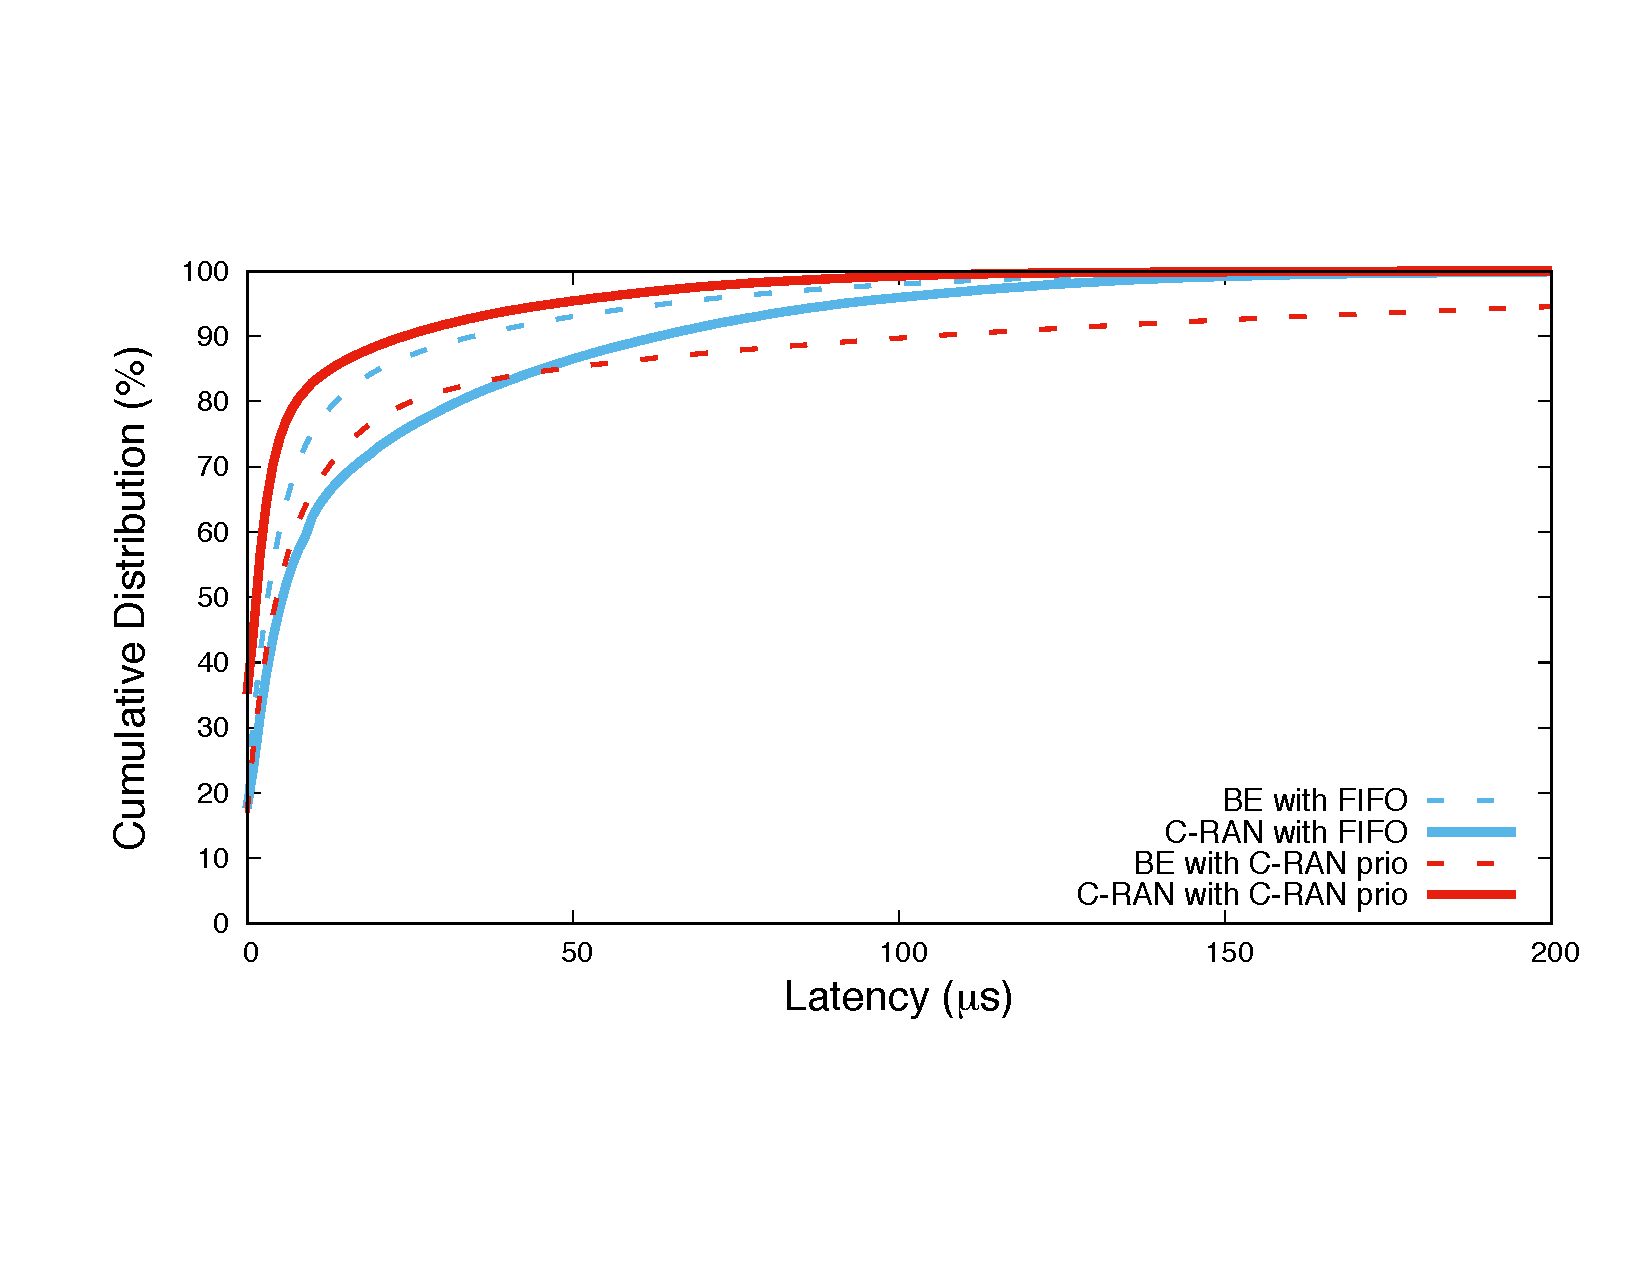
\includegraphics[scale=0.4]{opport}

 Cumulative distribution of the latency for different method in opportunistic insertion policy

\end{frame}

\begin{frame}{Slot reservation}

     \begin{minipage}[c]{0.4\linewidth}
        \begin{center}
      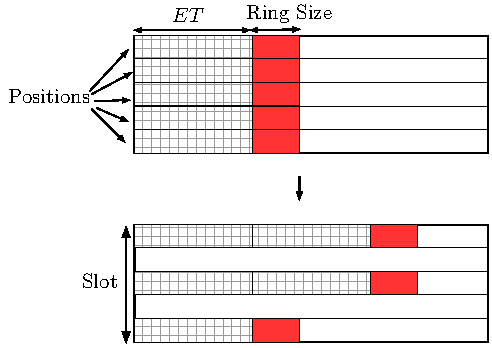
\includegraphics[scale=0.55]{repart2}
            \vspace{1cm}
      \captionof{figure}{Repartition in the slot}    \label{fig:repart1}
      \end{center} 
  \end{minipage}
  \hfill
    \begin{minipage}[c]{0.4\linewidth}
        \begin{center}
      \includegraphics[scale=0.55]{repart1}
      \vspace{1cm}
      \captionof{figure}{Repartition in the period}    \label{fig:repart2}
      \end{center} 
  \end{minipage}
\end{frame}

\begin{frame}{Slot reservation}

\centering
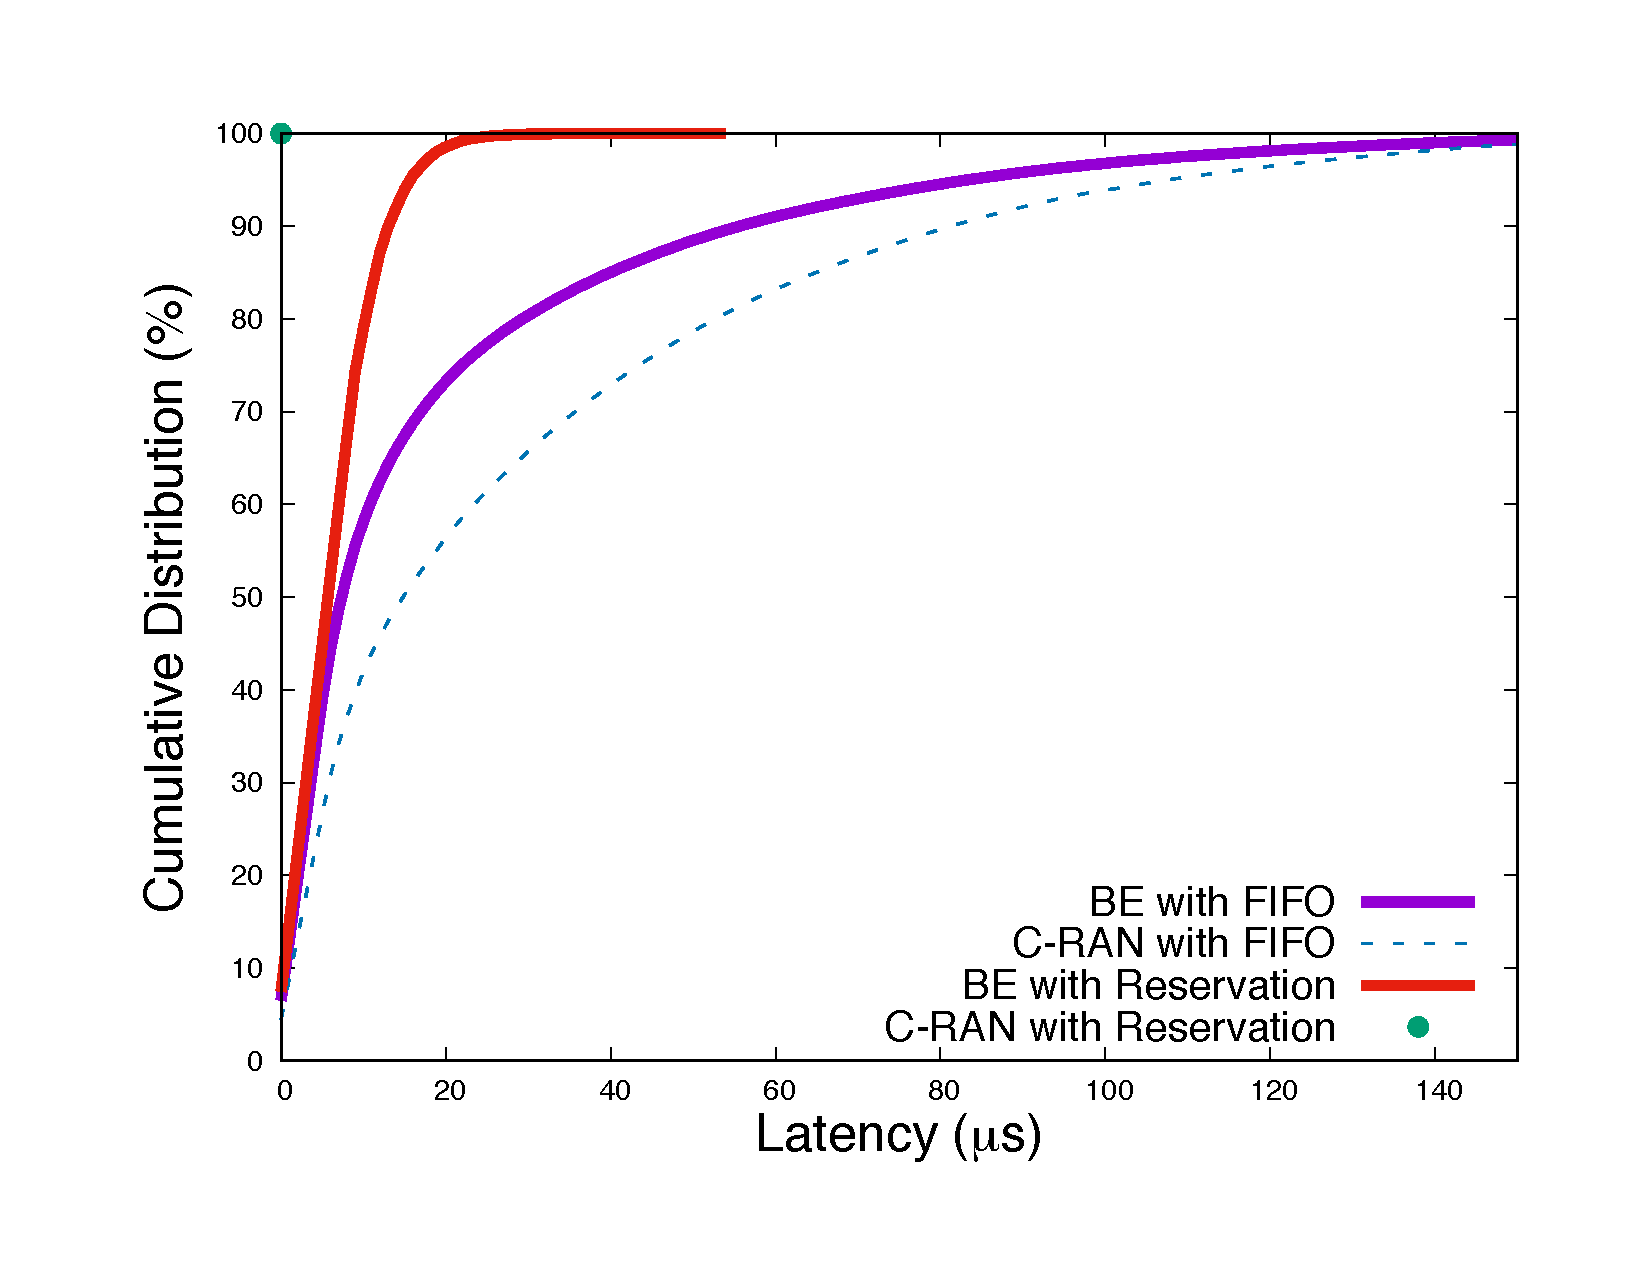
\includegraphics[scale=0.35]{optim}

 Cumulative distribution of the latency with slot reservation 

\end{frame}


\end{document}
